\documentclass{ltjbook}
\usepackage{docmute} 
\usepackage{../../myStyle} 

\begin{document}
\chapter{Multiple Regression Analysis}
\label{m10_MultipleRegression}

Last time, under the title "Regression Analysis," we discussed creating a prediction model based on the correlation between data. Predicting and controlling are fundamental to science, so it is wonderful to be able to do that.
However, since the data we use is intended for human subjects, it contains a lot of errors, so it doesn't fit perfectly like a theoretical model. Still, if an approximate linear function holds (if it appears to have a linear distribution), it can be very useful. That was the point we were trying to make.

This time, we will make the previous model a little more complex. In the previous model, we had $y=b_0+b_1x$, which was a simple model with only one explanatory variable $x$ for the explained variable $y$. This time, we will consider models with two or more explanatory variables.

\section{Multiple Regression Analysis}
The regression analysis with multiple explanatory variables is called \keytermE{Multiple Regression Analysis}. Note that this is distinct from \keytermE{Simple Linear Regression Analysis}, which involves only one explanatory variable. When there are multiple explanatory variables, say $x_1,x_2,\cdots,x_m$, they each have a coefficient assigned to them, denoted as $b_1,b_2,\cdots,b_m$. The intercept, however, remains the same as $b_0$. This can be represented by the following formula.

\[\hat{y_i}=b_0 + b_1x_{1i}+b_2x_{2i}+\cdots+b_mx_{mi}\]

There is a notation for explanatory variable, $x_{mi}$, which refers to the $i$th data point for the $m$th variable. The equation shown here is for the predicted value $\hat{y}$, but in reality, the observed value $y_i$ includes errors $e_i$ added to this prediction. The TeX code should not be altered.

\[ y_i = \hat{y_i} + e_i = b_0 + b_1x_{1i}+b_2x_{2i}+\cdots+b_mx_{mi} + e_i \]

I have prepared up to $x_m$ for general use, but for example, if it is two variables, it becomes $y_i = b_0 + b_1x_{1i}+b_2x_{2 i}+e_i$. Please make sure to carefully check where the $i$ is attached and where it is not attached.

Now, when we have $y=b_0+b_1 x$ (or the classic $y=ax+b$ form is also fine), the linearity model is discussed because it results in a straight line. When there are two explanatory variables, we plot it on a three-dimensional plane with three axes: the $x_1$ axis, the $x_2$ axis, and the dependent variable $y$ (Figure \ref{fig::10_01}). It is not feasible to illustrate when there are three or more explanatory variables. However, as an abstract and mathematical model, there is no problem with it. Also, the name remains the same even when it becomes a two-dimensional plane because it is still a straight line from a certain perspective. Therefore, regardless of the increase in the number of explanatory variables, it is generally known as \keytermE{linear regression} or \keytermE{linear model}.

\begin{figure}[ht]
   \centering
   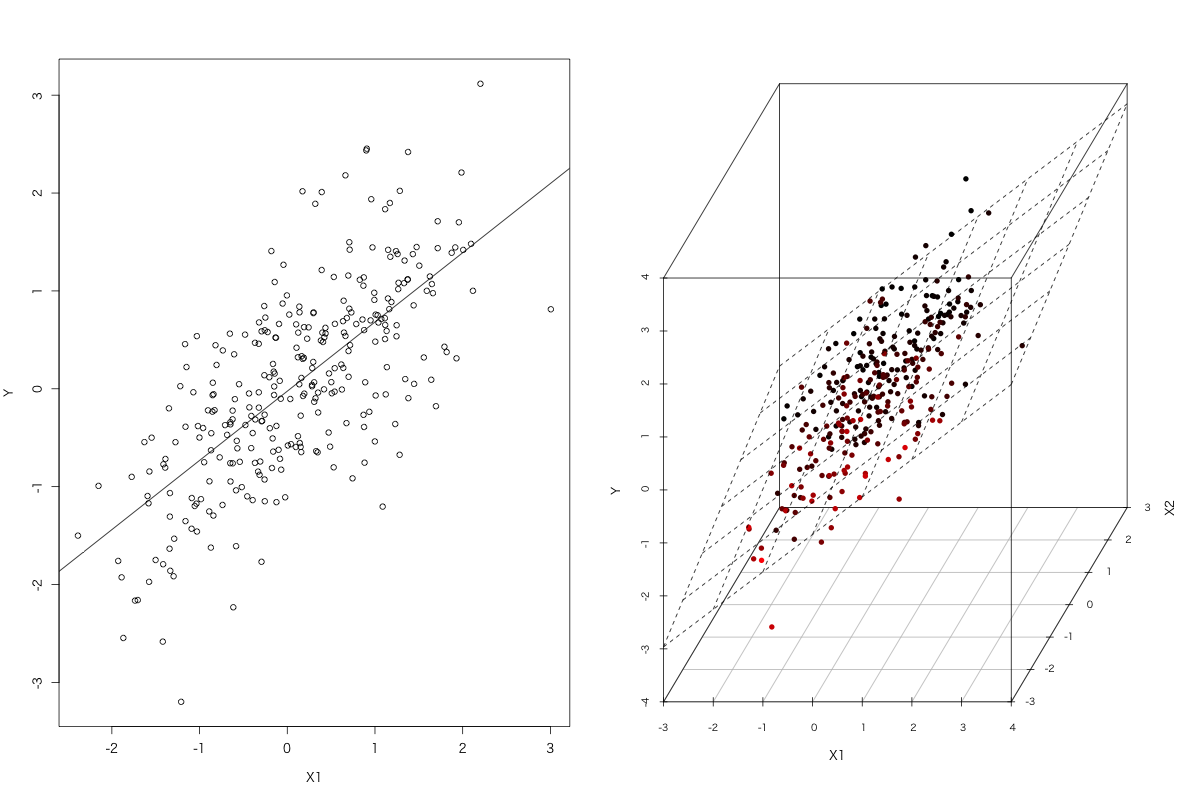
\includegraphics[keepaspectratio,width=0.65\linewidth]{../images/10_MultipleRegression/Rplot10_01.png}
   \caption{立体でも線形モデル}
   \label{fig::10_01}
\end{figure}


As the number of explanatory variables increases, calculating the regression coefficients becomes more complex. However, ultimately, using the same principle as the \keytermE{least squares method}, which is to determine the coefficients so that the error (variance) is minimized, it is possible to calculate the coefficients. Note that later on, other estimation methods/criteria such as the \keytermE{maximum likelihood method} and the \keytermE{Bayesian estimation method} that introduce the concepts of statistical inference and probability modeling will be introduced, but all of them are methods for solving unknown variables. Although the specific formula for calculation is not shown here, it is good to know that using R, you can get the answer in the same way as simple regression analysis.

Let's take a look at some specific numerical examples. Table \ref{tbl::10_01} includes data with an additional column compared to Table \ref{tbl09_01}. This time, it includes the average GPA, or the average score in university. It seems reasonable to consider that high school grades, university entrance exam scores, and university average scores all have an impact on the overall evaluation in university.

\begin{table}[ht]
   \caption{Example of high school and university grades 2}
   \centering
   \begin{tabular}[t]{rrrr}
      \hline
      Student ID & High School Transcript Score & University Entrance Exam Score & University GPA \\\hline
      \hline
      A    & 2.13   & 460     & 5.34   \\
      B    & 2.42   & 500     & 7.97   \\
      C    & 2.26   & 473     & 6.30   \\
      D    & 3.87   & 620     & 7.82   \\
      E    & 3.90   & 690     & 8.40   \\
      F    & 2.43   & 512     & 6.60   \\
      G    & 3.44   & 582     & 7.80   \\
      H    & 2.15   & 550     & 7.10   \\
      I    & 2.18   & 485     & 7.30   \\
      J    & 3.00   & 650     & 7.20   \\
      K    & 3.42   & 593     & 7.80   \\
      L    & 2.55   & 528     & 6.50   \\
      M    & 3.19   & 585     & 8.20   \\
      N    & 3.05   & 569     & 7.50   \\
      O    & 2.52   & 518     & 7.60   \\
      \hline
   \end{tabular}
   \label{tbl::10_01}
\end{table}

Once you have obtained this type of data, the next step is, of course, visualization. Creating a \textbf{picture of the data} is fundamental to analysis.

\begin{figure}[ht]
   \centering
   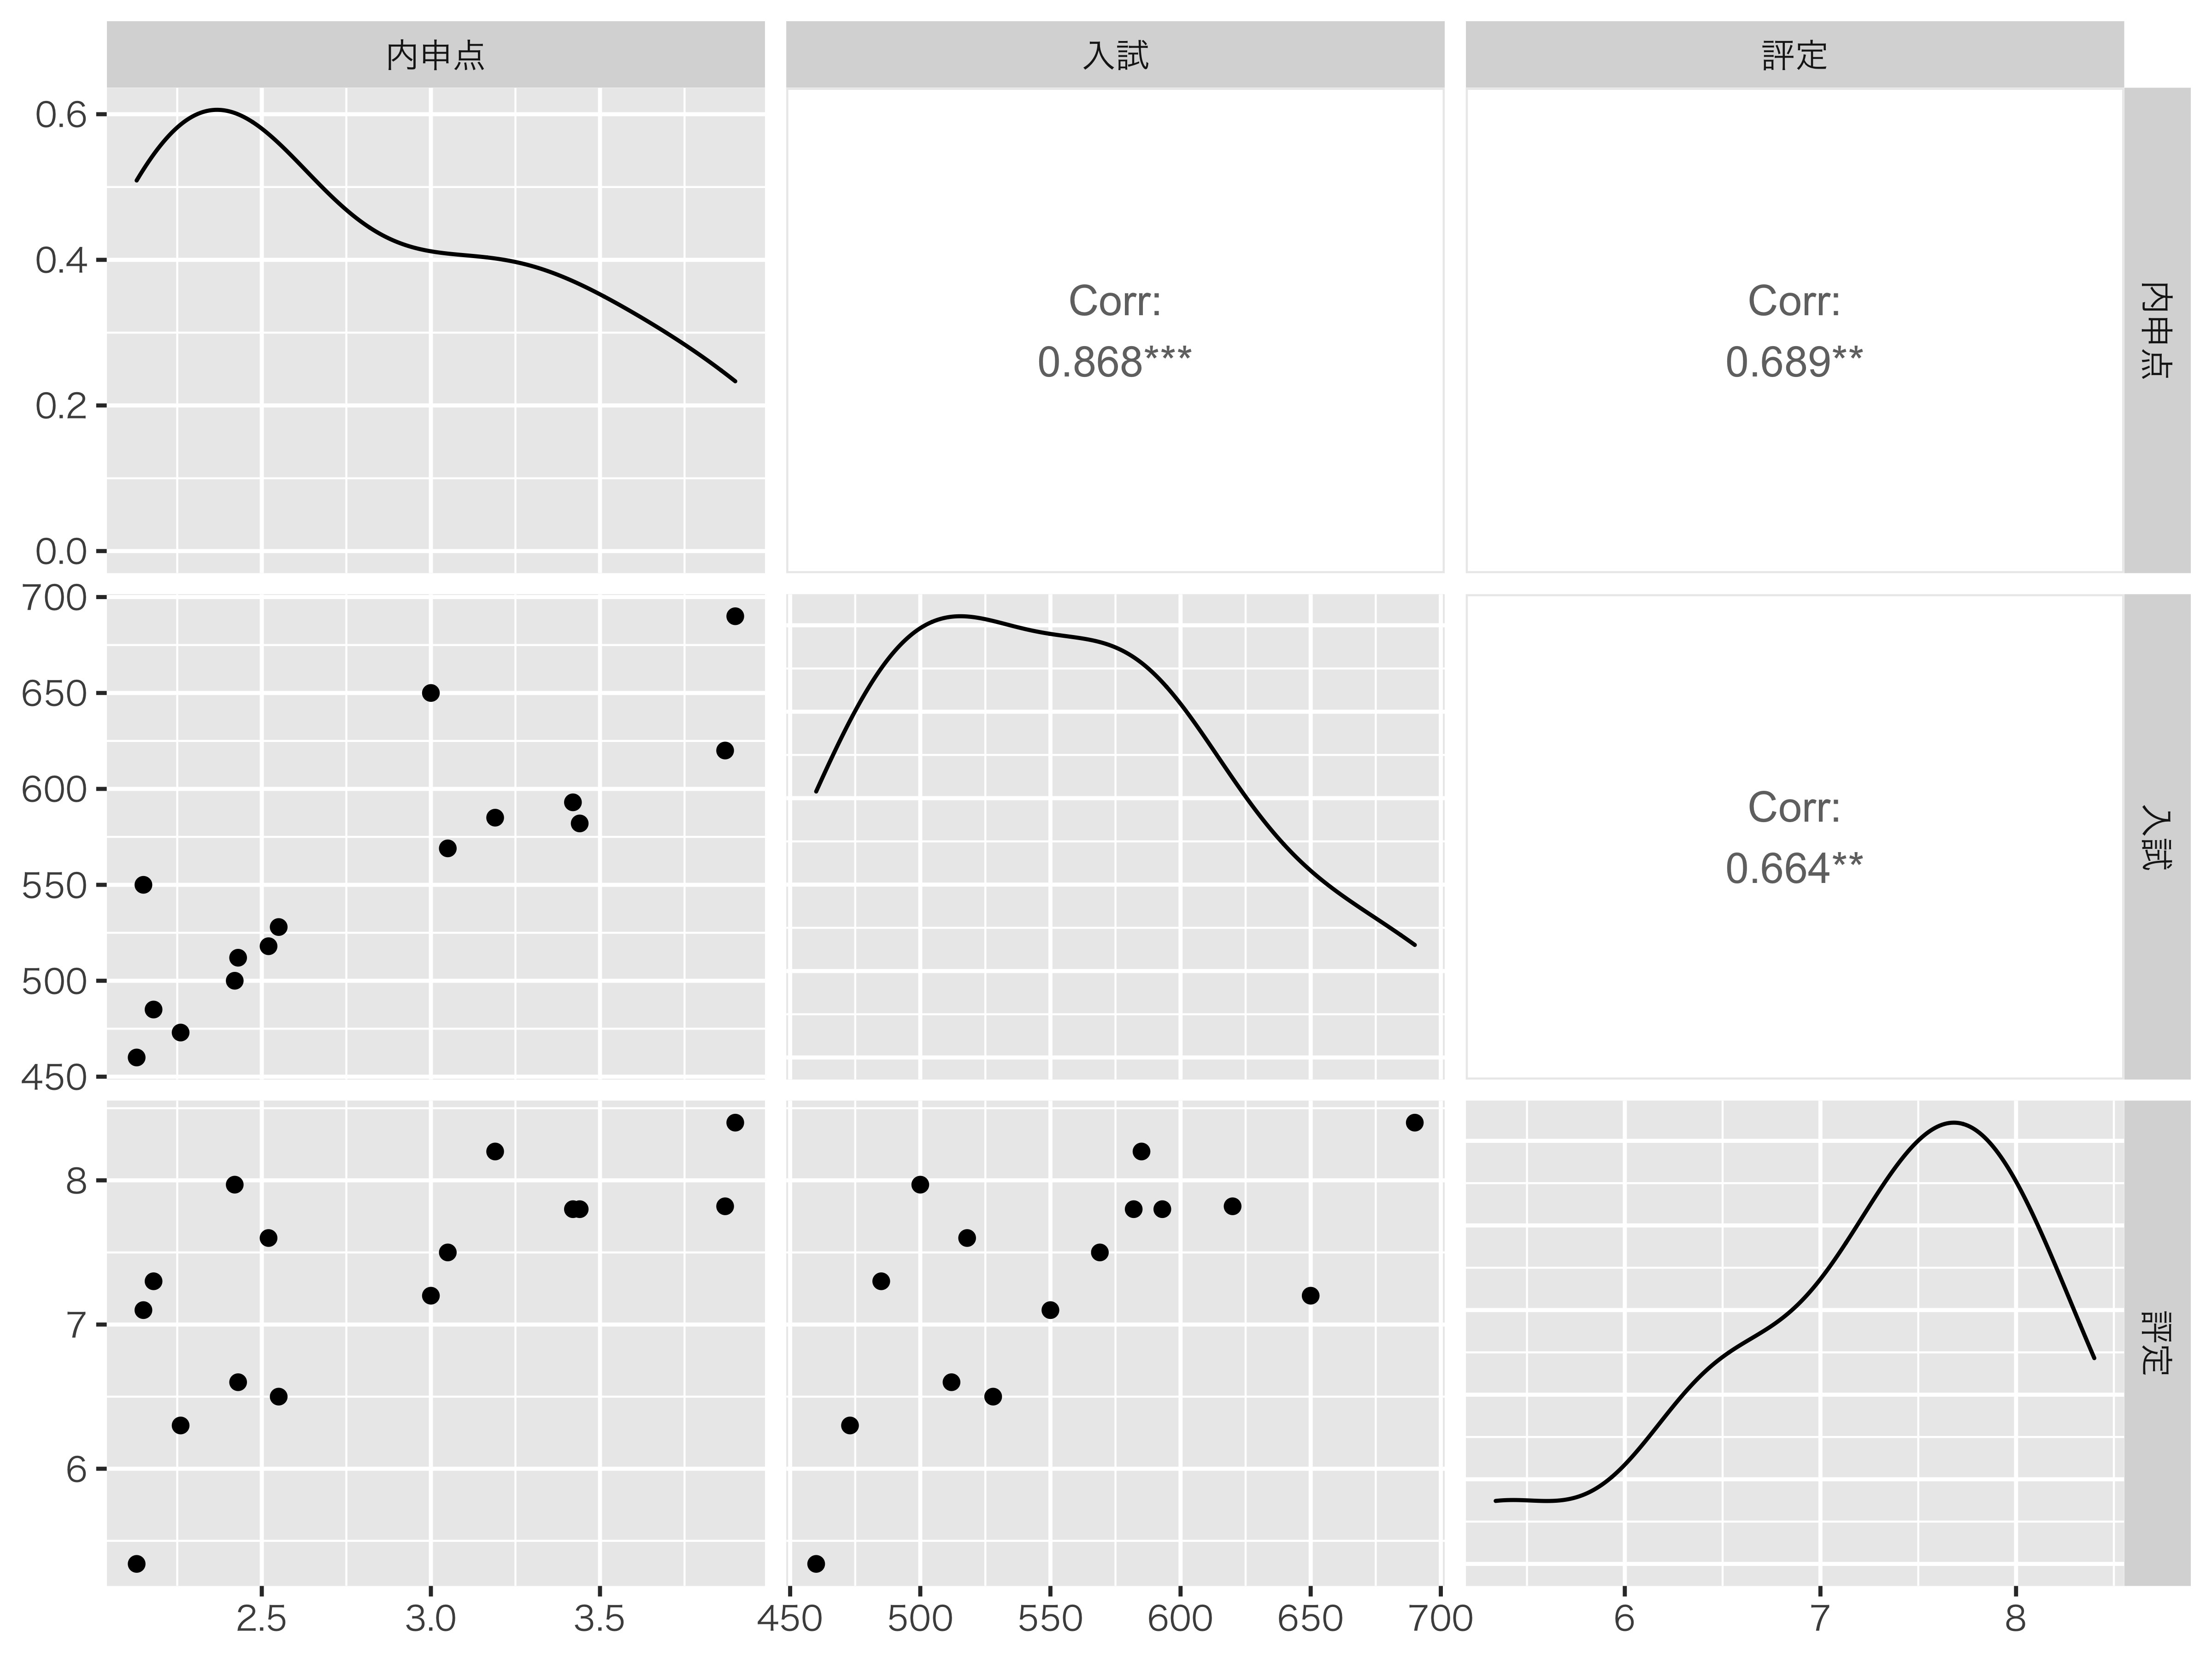
\includegraphics[keepaspectratio,width=0.65\linewidth]{../images/10_MultipleRegression/Rplot10_02.png}
   \caption{Visualization of variable relationships}
   \label{fig::10_02}
\end{figure}

Figure \ref{fig::10_02} shows a way to visualize data by arranging it in a $3\times3$ matrix. The rows contain the variables "internal score," "grades," and "GPA," and the columns contain the same variables. The diagonal cells (i.e. the cell at row n and column n) show graphs depicting the distribution of the data. The lower left cell shows scatter plots of two variable pairs, and the upper right cell shows their correlation coefficients. Although the information in the lower left and upper right cells is the same, it is presented visually and numerically, respectively. The TeX code is not modified.

When examining this data, there seems to be a significant correlation between the three variables. In particular, considering the average grade of the university as the dependent variable, there is a correlation of 0.689 between the internal assessment score and the average grade, and a correlation of 0.664 between the entrance exam and the average grade. Looking at the scatter plot, it also appears that both have a straight line relationship from the lower left to the upper right. Therefore, assuming the average grade as $y$, the internal assessment score as $x_1$, and the entrance exam score as $x_2$, let's try performing multiple regression analysis.

You can quickly calculate it in R, but leaving the details for another time, the result is the following regression equation.
\[ \hat{y} = 3.761+0.604x_1+0.003x_2 \]

In other words, if you multiply the school evaluation score by 0.604, multiply the entrance exam score by 0.003, and add 3.761, you can predict the average GPA of a university. For example, if someone has a school evaluation score of 2 points and an entrance exam score of 500 points, they would likely receive a score of around 6.469 by calculating 3.761 + 0.604 x 2 + 0.003 x 500.

Without altering the TeX code, please translate the following Japanese text into English:

また，仮想の値ではなく今回のデータを入れると，それぞれの予測値$\hat{y}$と，誤差の大きさが計算できます。

Furthermore, by inputting the current data instead of hypothetical values, it is possible to calculate each predicted value $\hat{y}$ and the amount of error.
I have put the predicted values in the \texttt{Yhat} column and the size of errors (residuals) in the \texttt{Residuals} column in Table \ref{tbl::10_02}.

The correlation coefficient between predicted values and actual dependent variables serves as an indicator of the model's \keytermE{goodness of fit}.
If we calculate the square of the correlation coefficient, known as the \keytermE{$R^2$ value}{R-squared value}, we obtain $R^2 = 0.9418$ for this data set. This means that about 95% of the post-enrollment grades can be predicted using the data from the entrance exams and the student's academic record.
\begin{table}[ht]
   \caption{Predicted values and residuals}
   \centering
   \begin{tabular}[t]{l|rrr|rr}
      \hline
      ID & Grades & Entrance Exam Scores & Ratings & Yhat     & Residuals  \\
      \hline
      A  & 2.13 & 460 & 5.34 & 6.560388 & -1.2203875 \\
      B  & 2.42 & 500 & 7.97 & 6.866879 & 1.1031209  \\
      C  & 2.26 & 473 & 6.30 & 6.681601 & -0.3816011 \\
      D  & 3.87 & 620 & 7.82 & 8.136849 & -0.3168493 \\
      E  & 3.90 & 690 & 8.40 & 8.384655 & 0.0153447  \\
      F  & 2.43 & 512 & 6.60 & 6.912295 & -0.3122954 \\
      G  & 3.44 & 582 & 7.80 & 7.752318 & 0.0476824  \\
      H  & 2.15 & 550 & 7.10 & 6.867773 & 0.2322275  \\
      I  & 2.18 & 485 & 7.30 & 6.672630 & 0.6273699  \\
      J  & 3.00 & 650 & 7.20 & 7.709539 & -0.5095393 \\
      K  & 3.42 & 593 & 7.80 & 7.776324 & 0.0236764  \\
      L  & 2.55 & 528 & 6.50 & 7.037309 & -0.5373092 \\
      M  & 3.19 & 585 & 8.20 & 7.611085 & 0.5889147  \\
      N  & 3.05 & 569 & 7.50 & 7.473985 & 0.0260146  \\
      O  & 2.52 & 518 & 7.60 & 6.986369 & 0.6136308  \\
      \hline
   \end{tabular}
   \label{tbl::10_02}
\end{table}


Multiple regression analysis is proving to be equally useful as simple regression analysis. However, it's important to be cautious when interpreting the results or expressing them in words.
Firstly, in terms of language, the regression coefficients of multiple regression analysis are particularly known as "partial regression coefficients". Although the character "partial" is used, this single character can be tricky.

In simple linear regression, the coefficient $b_1$ representing the slope indicates the growth rate of the dependent variable $y$ when the explanatory variable $x_1$ increases by one unit. That's what the slope means. For example, in the previous example where $\hat{y}=288.74+93.72x$, if the internal score of a student increases by one point, their entrance exam score is expected to increase by 93 points.

In this case, $\hat{y}=3.764+0.604x_1+0.003x_2$, which means "if your academic grade point average (GPA) goes up one point, your recommendation score (x1) will increase by 0.604, and if your entrance test score (x2) goes up one point, your GPA will increase by 0.003." However, it is important to note that "if your academic grade goes up one point" and "if your entrance test score goes up one point" are not completely independent. As shown in Figure \ref{fig::10_01}, the explanatory function in multiple regression analysis is a plane. When $x_1$ increases by one point, the image is that it moves horizontally in the direction of the $x_1$ axis, but $x_2$ does not change. Similarly, when $x_2$ increases by one point, the image is that it moves horizontally in the direction of the $x_2$ axis, but $x_1$ does not change.

By the way, please take a look at Figure \ref{fig::10_02}, which shows the original data. There is a correlation between the internal evaluation score and the entrance exam score, namely $x_1$ and $x_2$ ($r = 0.868$). This means that if $x_1$ changes, then $x_2$ will also change accordingly. It is like moving diagonally in the data space. Therefore, we cannot simply say that "if the internal evaluation score increases by one point...". The regression coefficient in multiple regression analysis represents the conditional coefficient of "if the entrance exam score is the same, then the internal evaluation score will increase by 0.604 points if it increases by one point". It is important to be aware of this and read on for a more detailed explanation.

\section{Partial correlation, partial correlation coefficient, and partial regression coefficient}
Please refer to Figure \ref{fig::10_03}, which is a scatter plot created from Table \ref{tbl::10_02} earlier.


\begin{figure}[ht]
   \centering
   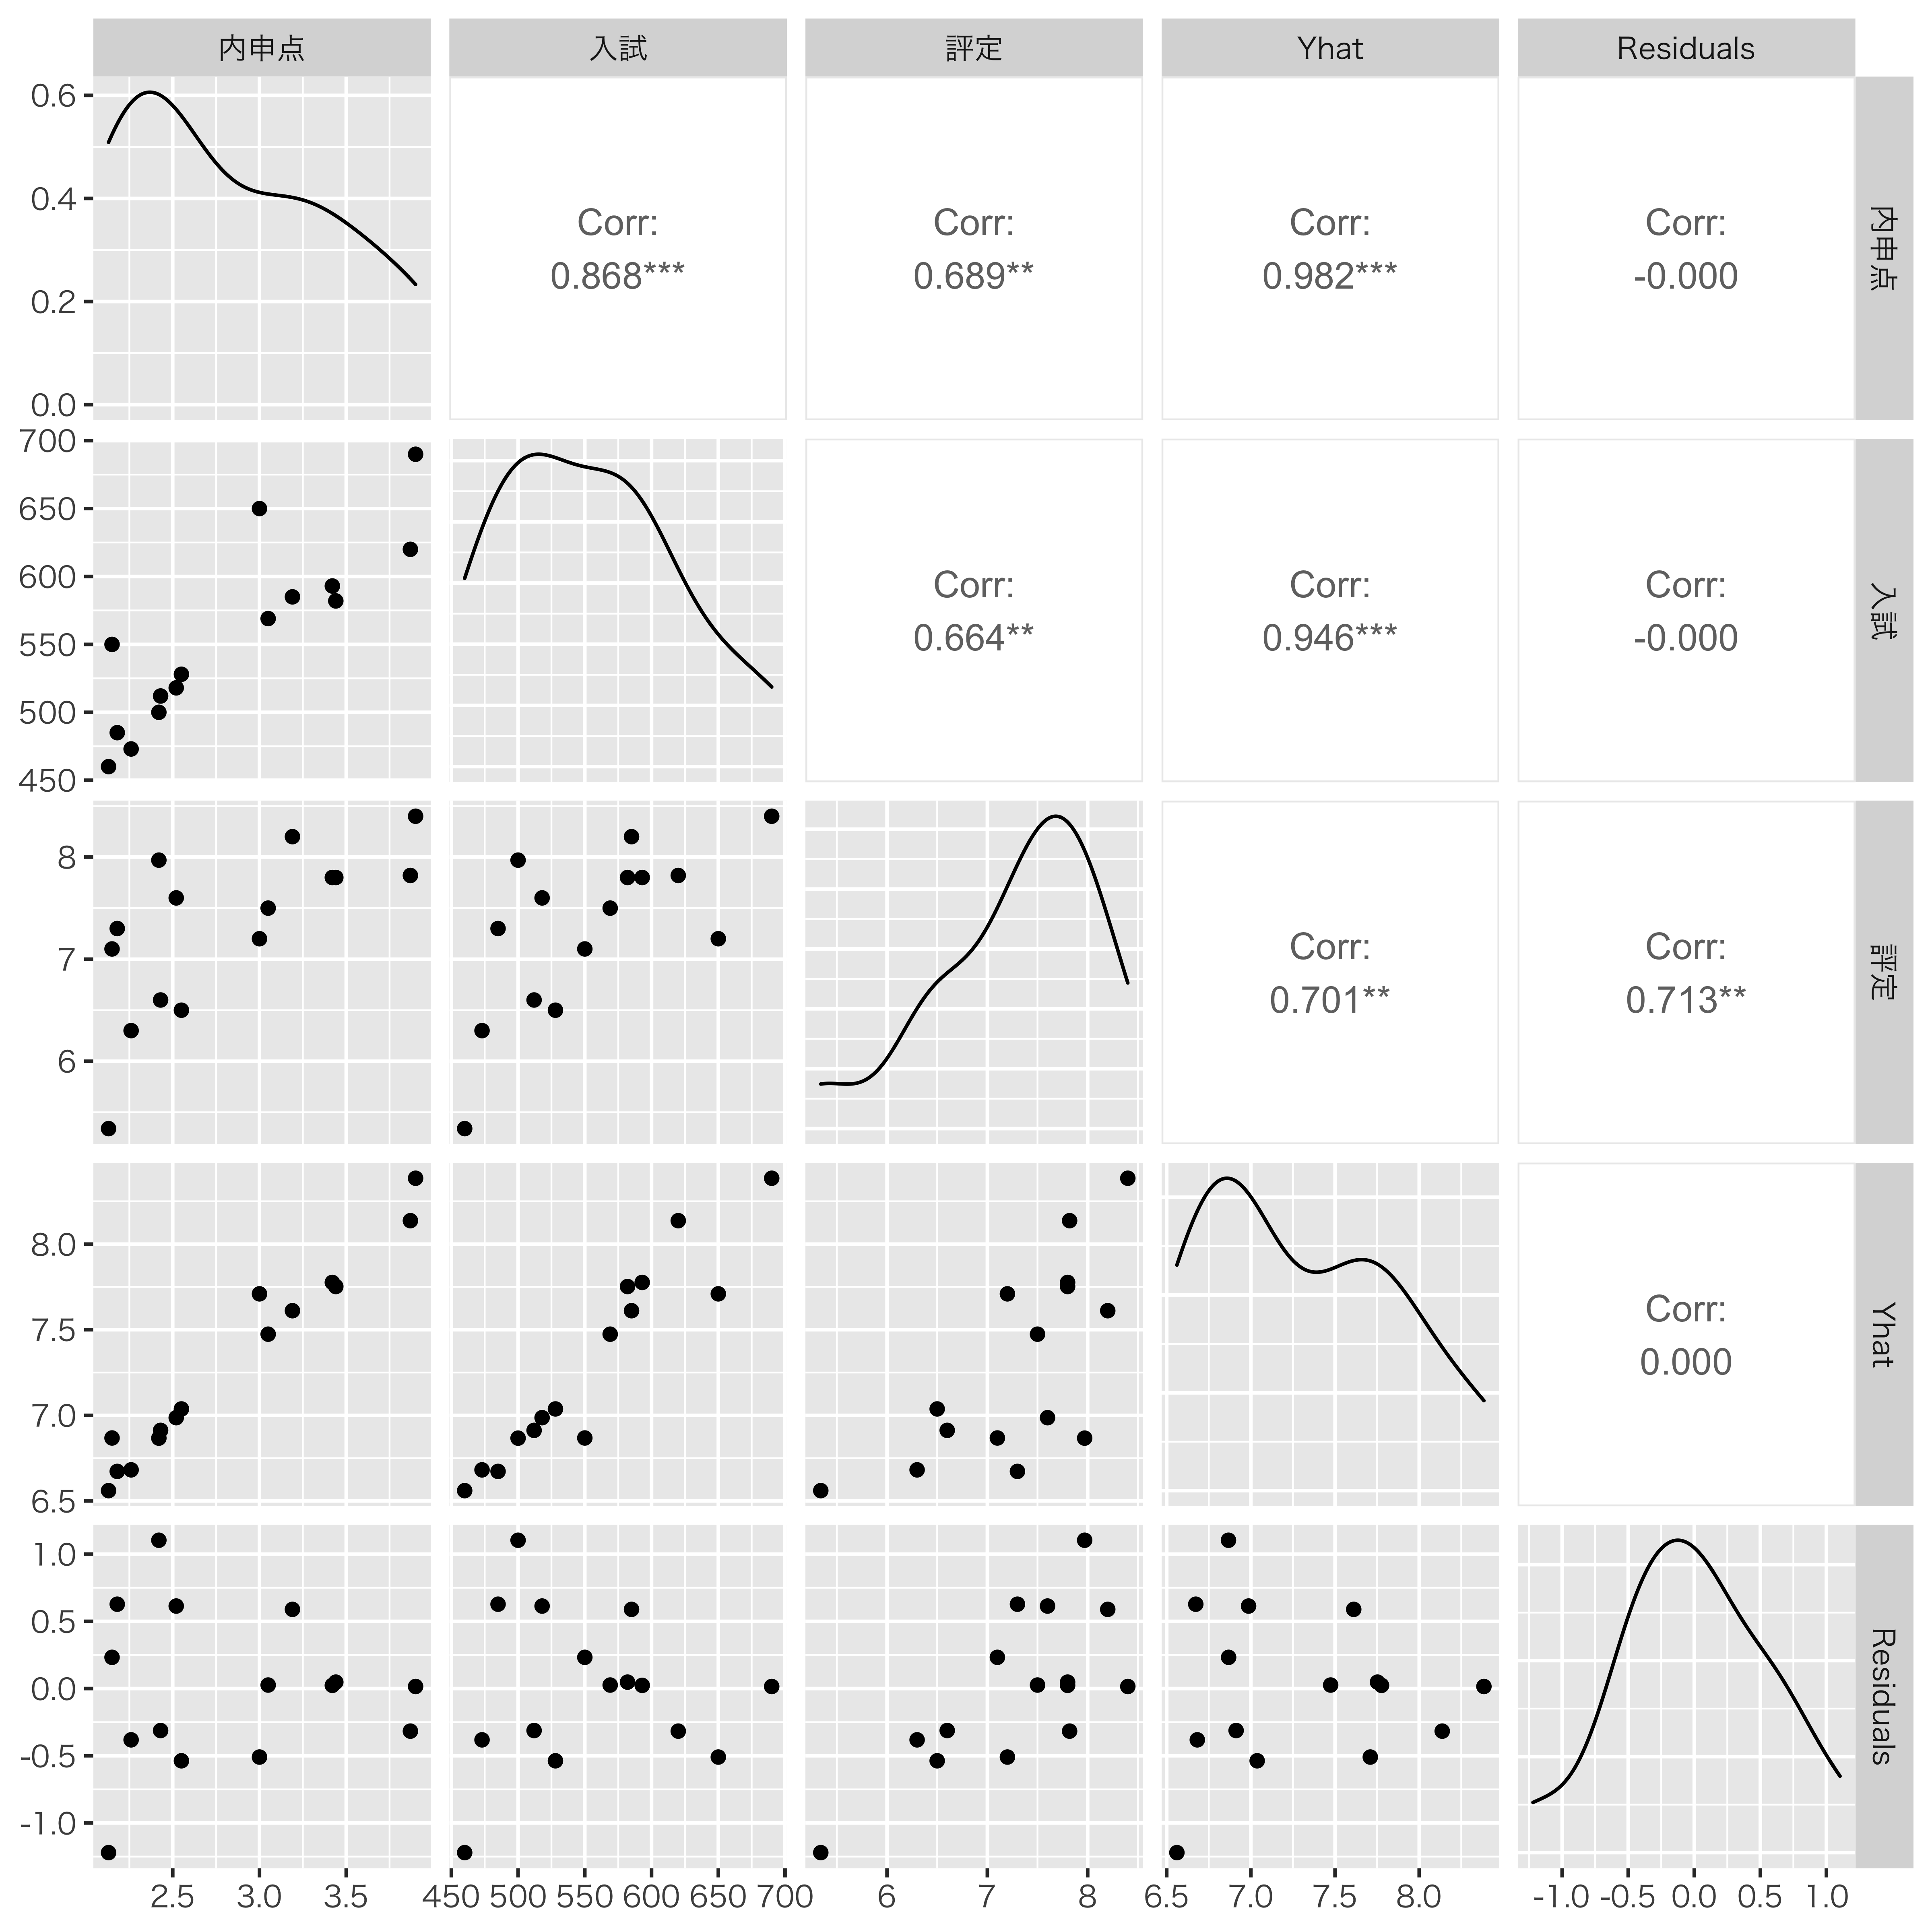
\includegraphics[keepaspectratio,width=0.75\linewidth]{../images/10_MultipleRegression/Rplot10_03.png}
   \caption{A scatter plot including predicted values and residuals.}
   \label{fig::10_03}
\end{figure}


Do you notice it? There is a point where the correlation coefficient is neatly $r=0.0$. Yes, the residuals $e_i$ and two explanatory variables $x_1$ and $x_2$ as well as the residuals $e$ and the predicted value $\hat{y}$ are all zero. This is not just a coincidence, but can be mathematically proven\footnote{Refer to \citet{kosugi2018}, Pp. 129--132 for details.}. Now we will think about what this means.

First, let's talk about the absence of correlation between residuals and explanatory variables. When regressing the dependent variable $y$ on an explanatory variable $x_1$, we can partition the variation in $y$ into the part that can be explained by $x_1$ and the part that cannot be explained by $x_1$ (see Figure \ref{fig::10_04}). The unexplained part is captured in the residuals $e$. If there is residual correlation with $x_1$, then there is room for improvement in the regression analysis. The regression coefficients are chosen to best fit the data, so there should be no principle correlation between $x_1$ and $e$. Figure \ref{fig::10_04} illustrates this concept.

\begin{figure}[ht]
   \centering
   
\includegraphics[keepaspectratio,width=0.75\linewidth]{../images/10_MultipleRegression/Slide10_01.png}
   \caption{Regression analysis divides the explanatory variables.}
   \label{fig::10_04}
\end{figure}


Now we can calculate the correlation coefficient for the other explanatory variable, $x_2$, along with the part that couldn't be explained by $x_1$. This correlation coefficient is called the \keytermE{semi-partial correlation coefficient}. You can understand this concept by looking at the diagram in Figure \ref{fig::10_05}.

\begin{figure}[ht]
	\centering
	
\includegraphics[keepaspectratio,width=0.75\linewidth]{../images/10_MultipleRegression/Slide10_02.png}
	\caption{Partial correlation coefficient}
	\label{fig::10_05}
\end{figure}


This refers to the partial correlation coefficient between the "university grade point average", which is the dependent variable, controlled by the first independent variable "high school academic performance" ($x_1$), and the "university entrance exam score" ($x_2$). When we say "controlled", we mean that the variable was controlled for or its influence was excluded. This is because we are looking at the correlation between the remaining unexplained factors and the variable after it has been explained by the academic performance ($x_1$), which can be interpreted as "excluded the influence of that variable"= "explained it to the fullest extent".

Furthermore, suppose we conduct a regression analysis with the second explanatory variable $x_2$ as the dependent variable, using the first explanatory variable $x_1$. In this case, the residuals can be considered as the influence of $x_1$ being removed from $x_2$. Using this method, we can conduct a regression analysis on both the entrance exam score ($x_2$) and the academic performance score ($y$) using the implicit score ($x_1$) to obtain the correlation coefficient of the residuals, which is referred to as the \textit{partial correlation coefficient}. This coefficient represents an unbiased correlation coefficient obtained by removing the influence of a variable from both variables. Figure \ref{fig::10_06} illustrates this idea.

\begin{figure}[ht]
	\centering
	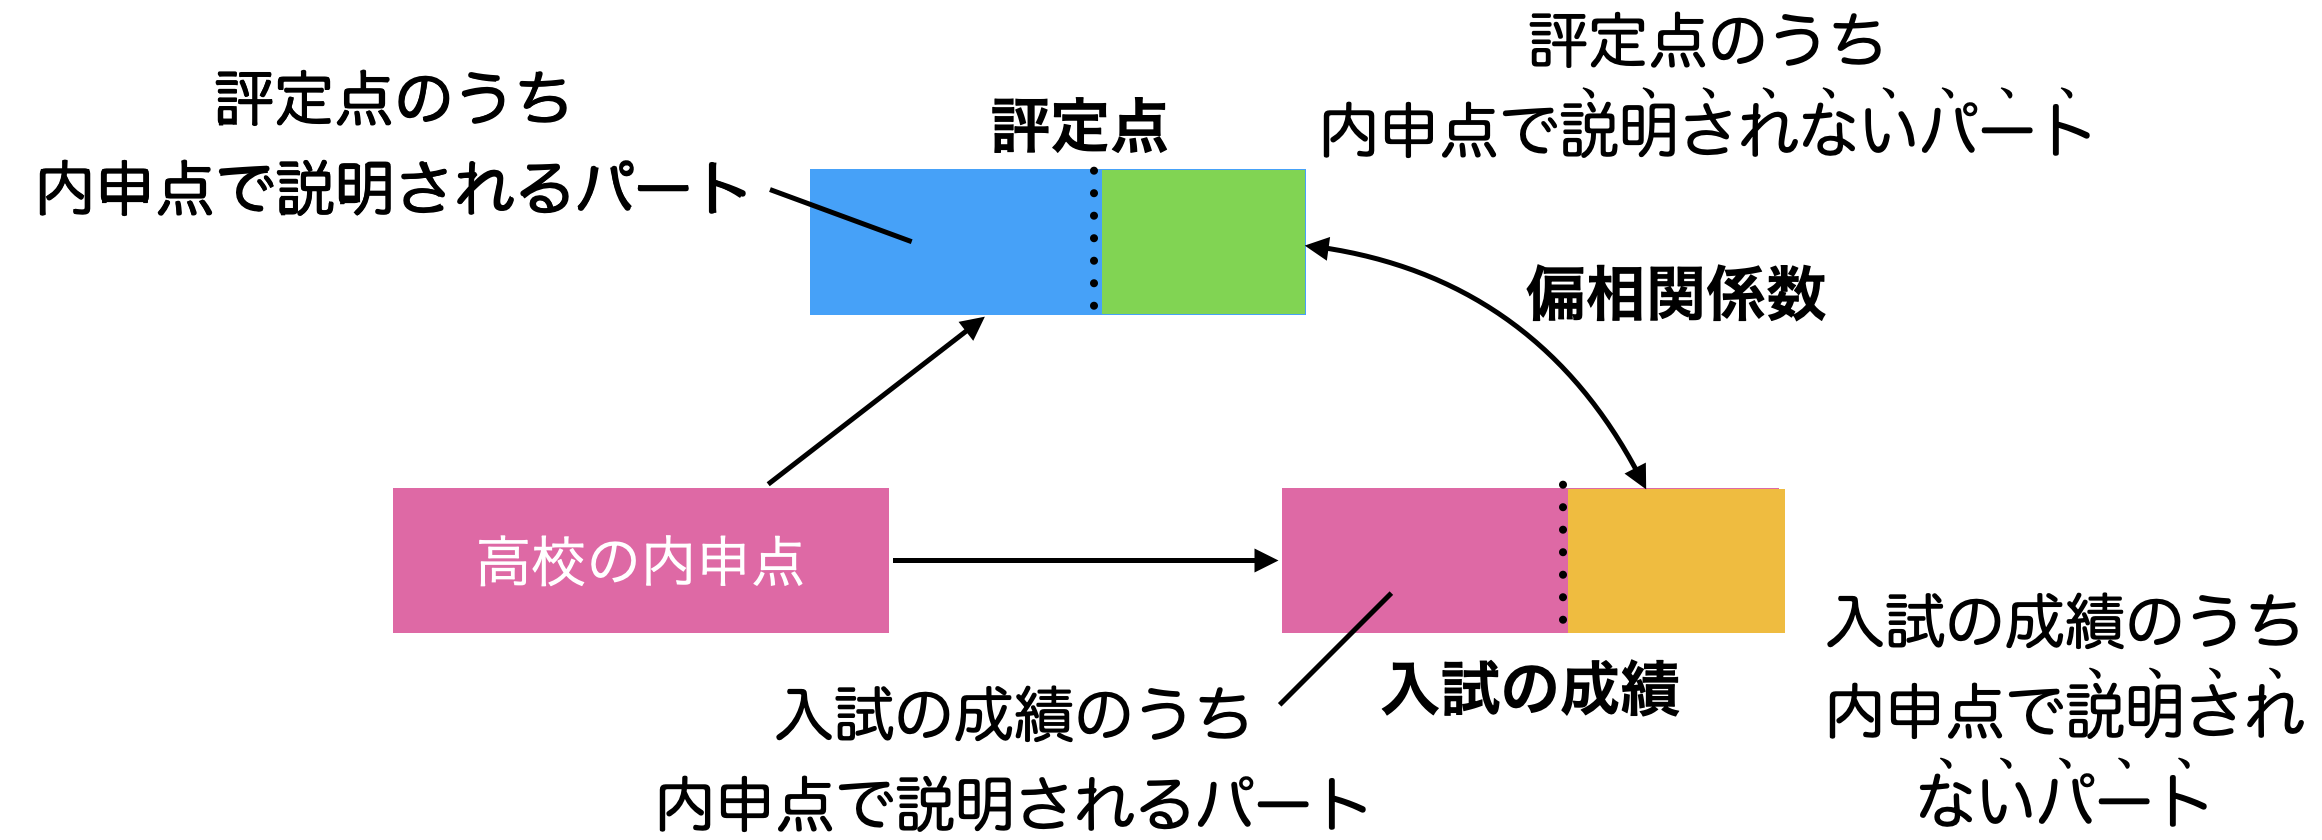
\includegraphics[keepaspectratio,width=0.75\linewidth]{../images/10_MultipleRegression/Slide10_03.png}
	\caption{Partial Correlation Coefficient}
	\label{fig::10_06}
\end{figure}



You can consider that there is a common factor of "high school grades" that affects both entrance examination results and college grades. In other words, even when you want to purely compare entrance examination results and college grades, the influence of underlying variables inevitably remains.
However, using this method allows us to see the pure "relationship between entrance exam scores and university grades" without the influence of underlying variables. This is amazing. For example, if you think about what else can predict the grade point average at the university, there are many things to consider. Some potential factors that could affect it are, for example, the time it takes to commute, whether the student has a part-time job, whether they are involved in a club, whether they have attended cram school in the past, and even the income level of their parents or the number of siblings they have. Moreover, this kind of information cannot be controlled at the survey stage. Even if you think that the amount of time spent studying differs depending on whether or not a student has a part-time job, it is difficult and costly to recruit only respondents who have a part-time job or only those who do not. Even if it can be controlled experimentally, there are too many variables to control in practice.

However, by digitizing various possible factors and performing regression analysis on them, and using the residuals of the rating average as a result, we can treat it as a factor that has been removed from various circumstances. By studying the residuals, we can say that we can neatly eliminate the effects of factors that cannot be controlled but must be considered! In the Residuals column of Table \ref {tbl :: 10_02}, there is information on the rating average at the university with the influence of two explanatory variables removed. Although the in-school grades and entrance examination scores vary from person to person, by removing their influence, we can consider the differences in rating averages.

Furthermore, we have investigated the correlation between $y$ and $x_2$ controlled by $x_1$, without altering the TeX code. However, using the residuals controlled by $x_2$ with $x_1$, we can also perform regression analysis on $y$ (Figure \ref{fig::10_07}). As a matter of fact, this is what is being calculated in multiple regression analysis, resulting in regression coefficients.
\begin{figure}[ht]
   \centering
   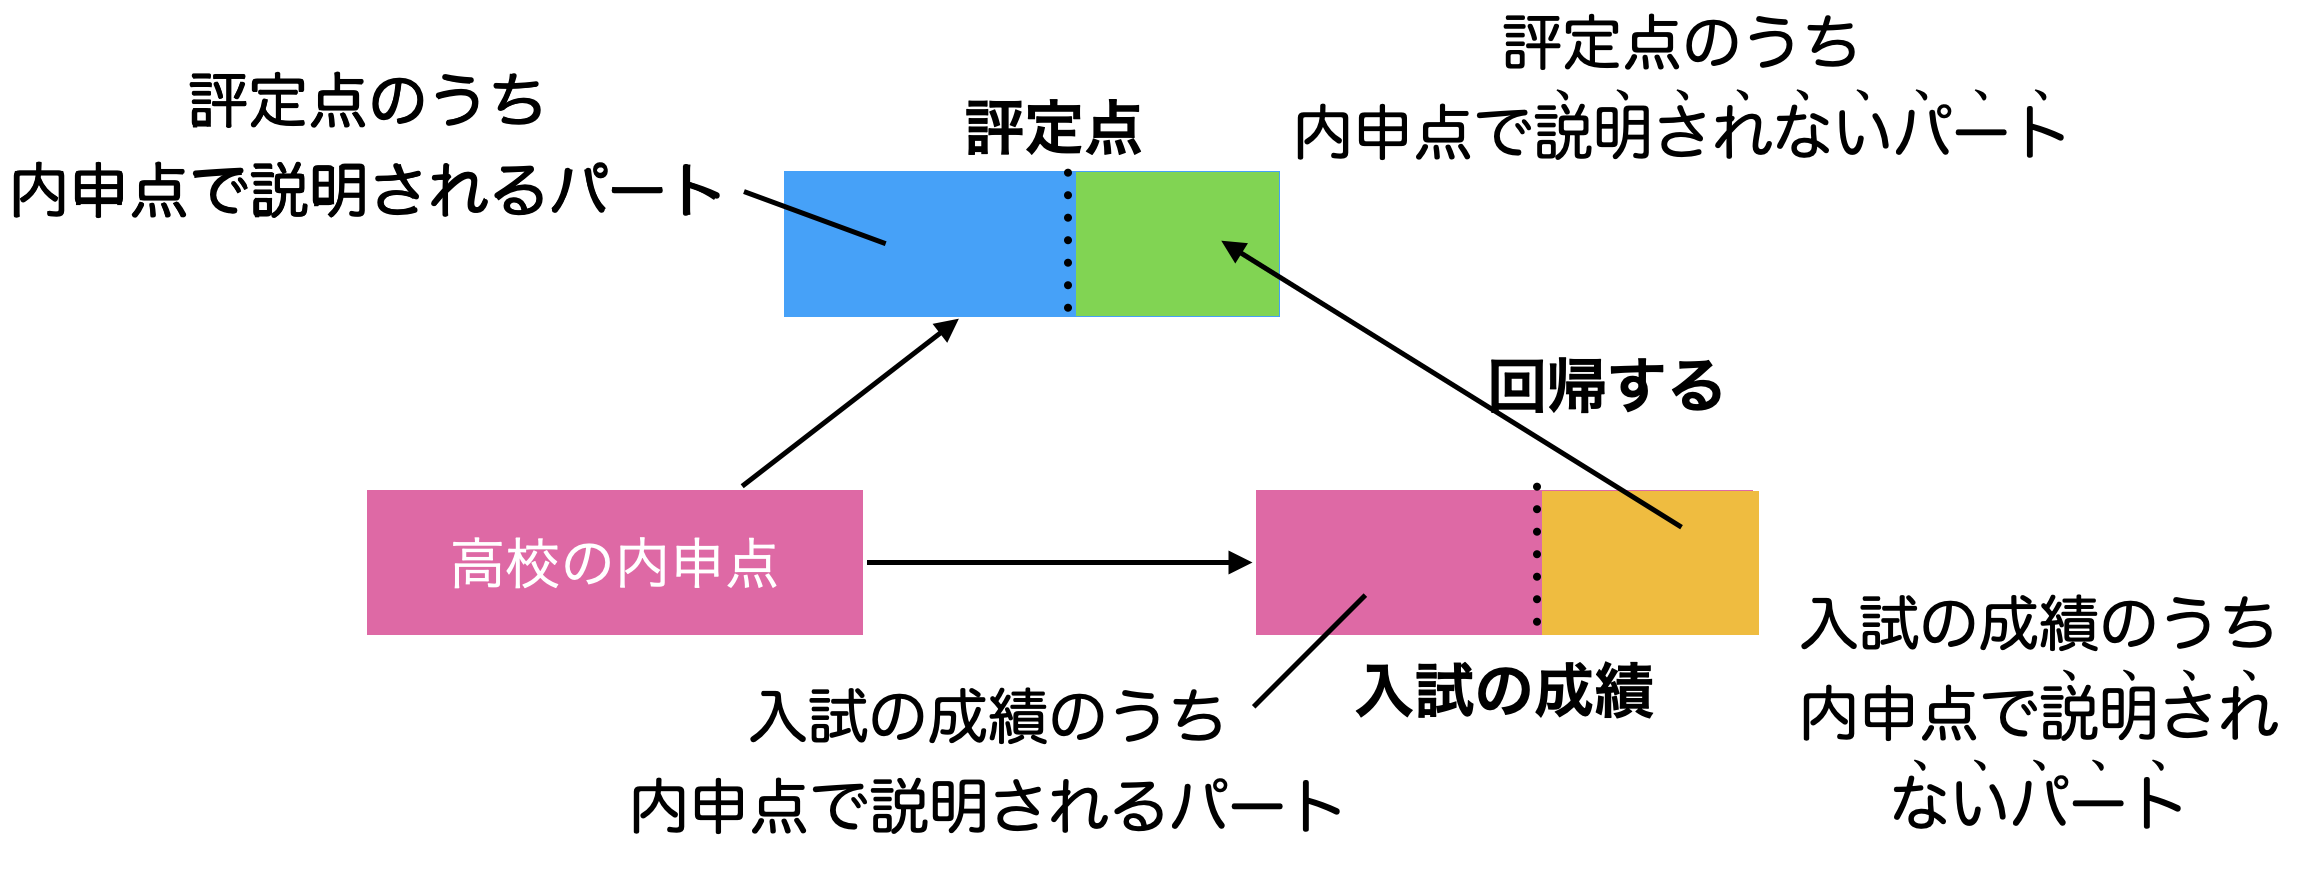
\includegraphics[keepaspectratio,width=0.75\linewidth]{../images/10_MultipleRegression/Slide10_04.png}
   \caption{Partial regression coefficients}
   \label{fig::10_07}
\end{figure}


The regression coefficients in multiple regression analysis are called \keytermE{partial regression coefficients}. The term "partial" is used because the influence of other variables has been removed. In the last section, we conveyed that the meaning of the regression coefficient is the rate of increase when moving horizontally along the $x_1$ and $x_2$ axes (Figure \ref{fig::10_08}). When interpreting the coefficient of $x_1$, it is important to note that $x_2$ is controlled (i.e. remains constant). To express it in words, it would be something like, "Assuming the entrance exam scores ($x_2$) are the same, if the academic record score ($x_1$) increases by one point, the post-entrance exam score ($y$) will increase by 0.604 points."
\begin{figure}[ht]
   \centering
   
\includegraphics[keepaspectratio,width=0.75\linewidth]{../images/10_MultipleRegression/Slide10_05.png}
   \caption{Meaning of the partial regression coefficient}
   \label{fig::10_08}
\end{figure}



"I imagine some people may find it a bit complicated and hard to understand what's wrong, so let's consider another example."
Let's say we gather data on the time spent on club activities $x_1$ and the time spent on part-time jobs $x_2$ to predict a university student's grades $y$. Please note that this is a hypothetical data for explanatory purposes and the TeX code will not be modified.
First, we conducted a simple regression analysis for each variable.
\[ \hat{y} = 2.8743 + 0.1407 x_1 \]
\[ \hat{y} = 15.4221 -0.5443 x_2 \]
I see. It can be interpreted that forming study groups leads to better grades (+0.1407), while working a part-time job leads to lower grades (-0.5443).

However, let's try multiple regression analysis here. We will include two variables in the prediction equation simultaneously.
\[\hat{y} = 21.9910 -0.1209 x_1 - 0.5956x_2\]
Oh, both coefficients turned out to be negative. The result shows that joining a club leads to lower grades and working a part-time job also leads to lower grades. Wasn't club activity supposed to be good? Why did such a reverse phenomenon occur?

Actually, there was a correlation between $x_1$ and $x_2$ in this data ($r_{12}=-0.4360$). It may be that there isn't enough time to work part-time while being involved in extracurricular activities, or vice versa. Either way, we can interpret that there is a negative correlation.
Also, the correlation with the explained variable is as follows: $r_{y1} = 0.1421, r_{y2} = -0.5529$. This trend is consistent with the results of simple regression analysis. It appears that people who spend a lot of time in the club tend to have high grades, while those who work longer hours at part-time jobs tend to have low grades.
However, it is important to note that there are hidden influences mixed in the direct relationship of $x_1 \to y$, $x_2 \to y$, which are not immediately apparent. In this case, since there is a relationship between $x_1$ and $x_2$, there is a route of influence known as the \keytermE{indirect effect} from $x_1 \to x_2 \to y$.

Multiple regression analysis shows the effects with indirect effects controlled. It is not the case that "if you spend more time on circle activities, your grades will drop, and if you spend more time on part-time jobs, your grades will also drop". Rather, the correct interpretation is "if the amount of time spent on part-time jobs is the same, spending more time on circle activities will result in lower grades" and "if the amount of time spent on circle activities is the same, spending more time on part-time jobs will also result in lower grades". Rather than drawing parallel conclusions where both factors are independent, we must interpret this conditionally.
Also, of course, if you haven't researched the issue of work hours, you might come to the conclusion that "joining a club is good, as data shows that grades improve." When conducting analysis, it's important to consider all variables that could potentially impact the dependent variable, otherwise you may end up with incorrect conclusions.

As we saw earlier, the simple correlation coefficient $r_{y1}$ must be carefully controlled and evaluated as it includes both the direct effect (partial correlation coefficient) and the mixed indirect effects. When interpreting the results of multiple regression analysis, we must also be mindful of this expression.

Furthermore, when there is a strong correlation between explanatory variables, the results of multiple regression analysis itself can be inaccurate. This problem is called \keytermE{multi-collinearity}, which particularly arises when $x_1$ and $x_2$ have a strong correlation coefficient such as $r_{12}=0.9$ or close to $1.0$.
It feels like one could say "$x_1 \simeq x_2". If we try replacing $x_2$ with $x_1", the regression equation becomes as follows:
\[ \hat{y} = b_0 + b_1 x_1 + b_2x_2 \]
Here, since $x_1 \simeq x_2$, which is almost the same, let's replace it with $x_1=x_2$.
\[ \hat{y} = b_0 + b_1 x_1 + b_2x_1 \]
The coefficients are combined as follows.
\[ \hat{y} = b_0 + (b_1+b_2) x_1 \]
The final equation has the same form as a simple regression analysis. As there is only one coefficient in simple regression analysis, there are infinite pairs of coefficients $b_1$ and $b_2$ that satisfy the equation $b_s = b_1 + b_2$, and the solution is not unique. In practice, it is unlikely that $x_1$ and $x_2$ are replaced by each other, but the same problem occurs when the correlation is high. When multicollinearity occurs, problems arise where the sign of the regression coefficient ends up being the opposite of the true relationship, resulting in incorrect answers.

When there is a correlation between explanatory variables, it is important to be particularly careful. While multiple regression analysis is very simple when there is no correlation between explanatory variables, this is not always the case in practice. To ensure proper interpretation and account for multicollinearity, it is advisable to first visualize the data and check whether there is a correlation between explanatory variables.


\section{Standardized Coefficients}

Now, going back to our discussion, I would like to review the regression equation that predicts a university's grade point average $y$ based on the high school's recommendation score $x_1$ and entrance exam score $x_2$ without modifying the TeX code.

\[ \hat{y} = 3.761+0.604x_1+0.003x_2 \]

Looking at these numbers, the regression coefficient for high school grades is 0.604 and the regression coefficient for entrance exam scores is 0.003. From these two numbers, it appears that entrance exam scores are relatively insignificant. Does this mean that high school grades are 200 times more important than entrance exam scores? Actually, no. In this case, the dependent variable has a minimum value of 5.340 and a maximum value of 8.385. The explanatory variables are stretched (through multiplication by the coefficients) or shifted (through addition of the intercept) to fit this dependent variable. For high school grades, which have a minimum value of 2.13 and a maximum value of 3.90, a simple stretch of the data suffices to fit within the range of 5 to 8. However, entrance exam scores have a minimum value of 460 and a maximum value of 690. To fit within the range of 5 to 8, which is an order of magnitude smaller than the original range, a scaling down of approximately 1/100 is necessary. Therefore, the coefficient for $x_2$ is very small and expressed as a decimal.

In expressions using raw data like this, we cannot directly compare the partial regression coefficients if the units are different, because the relative influence cannot be judged by comparing them as they are. So what should we do? Since we cannot make a relative comparison because the units are different, we can make a relative comparison by removing the units. Yes, this operation is called \textit{standardization}.

The explanatory variables and dependent variables both have units attached, so to align them, each variable is standardized. The standardized dataset appears as shown in Table \ref{tbl::10_03}.

\begin{table}[ht]
	\caption{Standardized data (partial)}
	\centering
	\begin{tabular}[t]{l|ccc}
		\hline
		ID       & Academic Record Score z & Admission Exam Score z & Evaluation Score z \\
		\hline
		A        & -1.1382198              & -1.4131716             & -2.3874746         \\
		B        & -0.6693508              & -0.8139469             & 0.8237724          \\
		C        & -0.9280371              & -1.2184236             & -1.2153084         \\
		D        & 1.6749939               & 0.9837272              & 0.6406214          \\
		N        & 0.3492265               & 0.2197157              & 0.2498993          \\
		$\vdots$ & $\vdots$                & $\vdots$               & $\vdots$           \\
		O        & -0.5076719              & -0.5442958             & 0.3720000          \\
		\hline
	\end{tabular}
	\label{tbl::10_03}
\end{table}


This standardized dataset has each variable with a mean of 0 and a variance of 1, allowing for relative comparisons as-is. When conducting regression analysis using this dataset, the resulting output would be as follows.

\[ \hat{y.z_i} = 0.4564 x.z_{1i} + 0.2674 x.z_{2i} \]

The standardized regression coefficient for academic performance was 0.4564, while the standardized regression coefficient for entrance exam scores was 0.2674. By comparing these, it is possible to correctly determine that academic performance has a greater influence than entrance exams. The partial regression coefficients for each variable, calculated by standardizing them, are called \textit{standardized partial regression coefficients}. Although the name is long, it can be understood when you think about its meaning. The standardized partial regression coefficient represents the coefficient that indicates how much the dependent variable changes when the independent variable, $x_1$, increases by 1 SD when $x_2$ score remains constant. The interpretation may not be straightforward. The unstandardized regression coefficient was easier to understand because it had units, but it was difficult to compare, while the standardized regression coefficient has no units, which makes it more difficult to understand but easier to compare.

Let me mention two more characteristics when performing regression analysis with standardized scores.
The first thing to note is that there is no value for the intercept $b_0$. Have you noticed? The intercept term is used for adjusting the overall height of variables and is calculated taking into account the average value of each variable, but when using standardized data, the mean of all variables is zero, so this adjustment is no longer necessary. Therefore, in the case of standardization in regression analysis, it is natural that there is no intercept.
Let's consider another aspect of model fit. Actually, the $R^2$ values remain the same whether the data is standardized or not. Whether the data is standardized or not, there is no change in the variable relationships (correlation) when fitting a linear model. Only the position and scale changes, and the appearance of the scatter plot does not change. It is an obvious thing when you think about it, but it is worth confirming again.


\section{Summary for Today}
\begin{itemize}
	\item Multiple explanatory variables regression analysis is called multiple regression analysis. The regression coefficients at this time are called partial regression coefficients.
	\item Please note that the partial regression coefficient is the "regression coefficient when controlling other variables". Let's understand the partial correlation coefficient, the partial correlation coefficient, and the partial regression coefficient in that order.
	\item When there are multiple explanatory variables, the units are different, so use standardized partial regression coefficients to compare the influences with each other.
\end{itemize}


\section{Task}

I collected data from about 8 properties in the vicinity of the university to investigate the market rate of one-room apartments (see Table \ref{tab:ex11_01} and Figure \ref{fig::10_08b}). Based on this, I conducted multiple regression analysis with rent as the dependent variable and size, age of the building, and travel time from the nearest transportation as independent variables.

\begin{table}[ht]
	\caption{Rent Data}
	\label{tab:ex11_01}
	\centering
	\begin{tabular}[t]{rrrr}
		\hline
		Area (square meters) & Age of Building & Distance from Station (minutes on foot) & Rent \\\hline
		41.40                & 14              & 10                                      & 8.60 \\
		20.28                & 16              & 9                                       & 6.10 \\
		18.20                & 28              & 10                                      & 4.20 \\
		19.87                & 16              & 13                                      & 5.70 \\
		20.28                & 19              & 7                                       & 6.30 \\
		23.18                & 20              & 14                                      & 5.40 \\
		19.87                & 17              & 12                                      & 6.25 \\
		19.87                & 20              & 17                                      & 5.80 \\
		\hline
	\end{tabular}
\end{table}



\begin{figure}[ht]
	\centering
	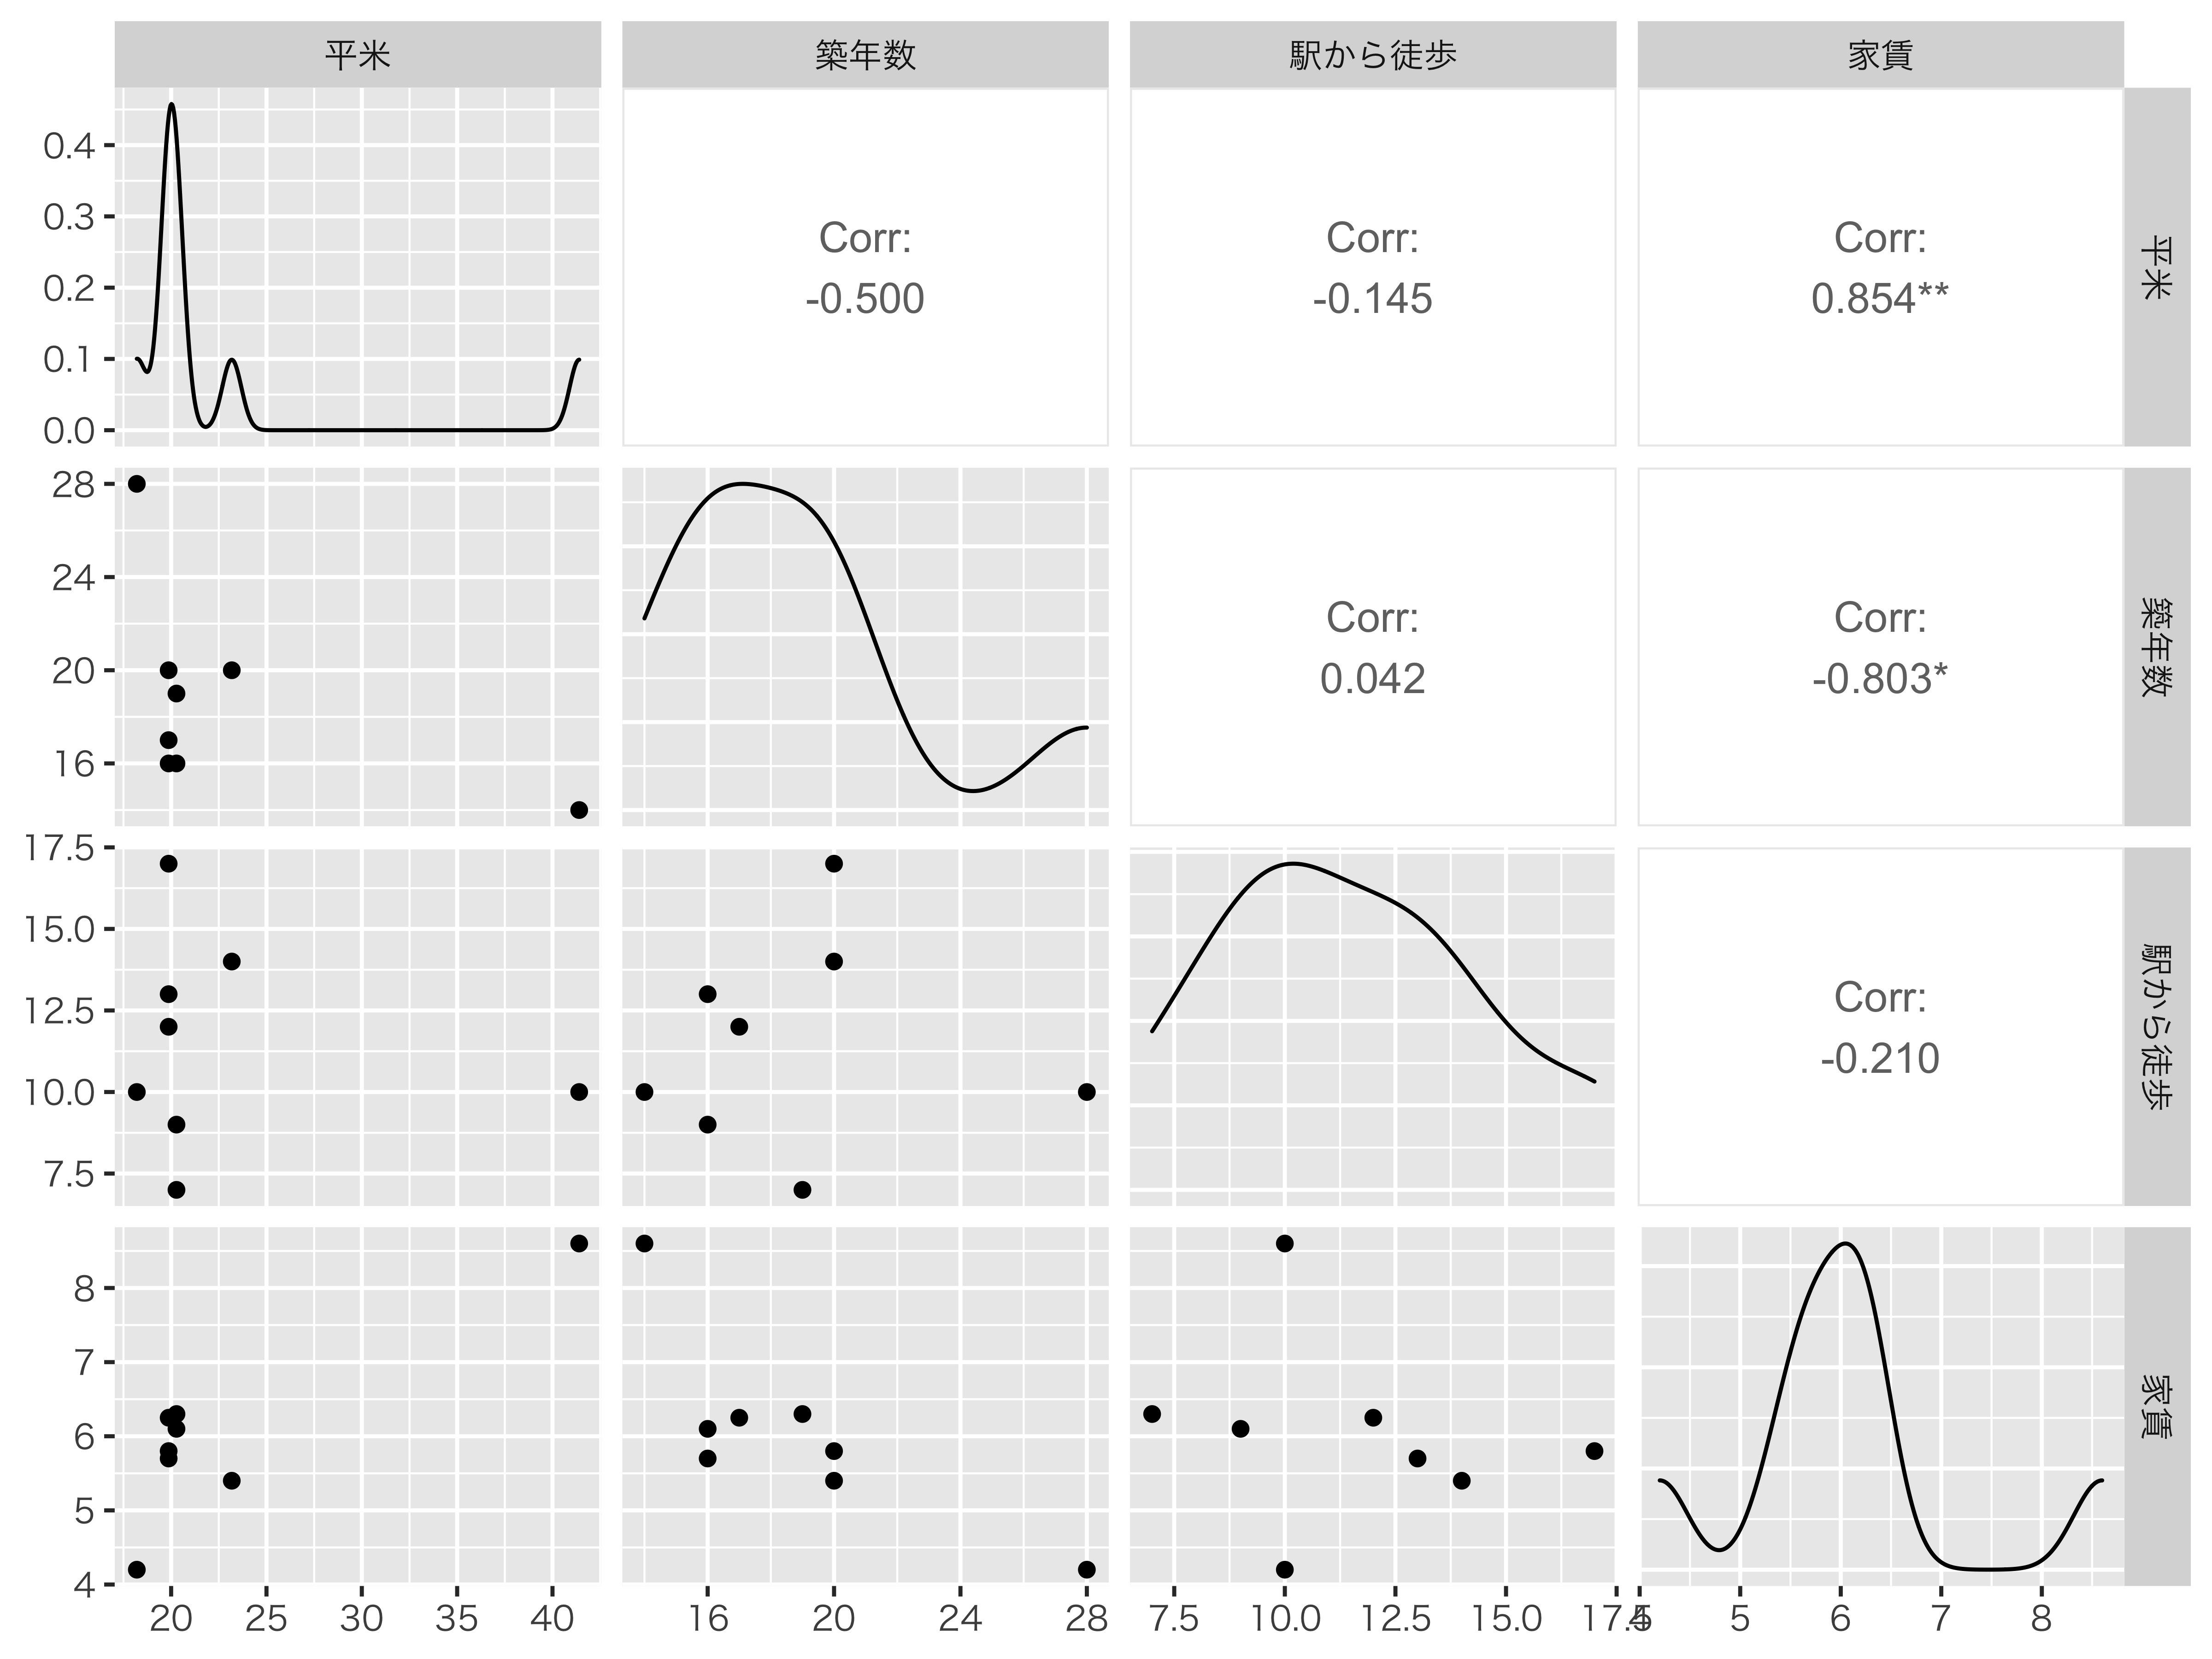
\includegraphics[keepaspectratio,width=0.65\linewidth]{../images/10_MultipleRegression/Rplot10_04.png}
	\caption{Plot of sample data}
	\label{fig::10_08b}
\end{figure}


The multiple regression equation for raw data is:
\[ \mbox{Predicted Value}　＝　7.05　+　0.09\mbox{square meters}　-　0.14\mbox{years since construction}　-　0.04\mbox{commuting time} \]

The multiple regression equation for the standardized data with each variable standardized is as follows:
\[ \mbox{Estimated Value} = 0.58\text{ square meters} - 0.51\text{ years old} - 0.10\text{ commuting time} \]

It became as follows. In addition, the goodness-of-fit index was $R^2=0.93$.

Please answer the following questions based on the data and results presented.

\paragraph{Understanding the Results of Multiple Regression Analysis 1} Please check all the options that correctly express the regression analysis of raw data and its results. (Note: The TeX code should not be modified.)
\begin{itemize}
   \item The intercept is 7.05.
   \item If the moving time is the same, the rent is 1400 yen lower for every one-year increase in age for the same property.
   \item The most important variable in determining rent cannot be determined by regression analysis.
   \item The most important variable in determining rent is the age with the largest absolute value coefficient.
   \item The most important variable in determining rent is the positive square meter coefficient.
   \item If the moving time and age are the same, the rent is 900 yen higher for every one square meter increase.
   \item For every one year increase in age, the rent decreases by 1400 yen.
   \item Due to high correlation coefficients between the dependent variables, rent and square meters or rent and age, it is necessary to suspect multicollinearity. 
\end{itemize}


\paragraph{Understanding the Results of Multiple Regression Analysis 2} Please check all of the following expressions that correctly represent the regression analysis and its results for standardized data.
\begin{itemize}
   \item If the moving time and age of the property are the same, the rent increases by 5800 yen per square meter.
   \item The most important variable in determining rent cannot be determined from regression analysis.
   \item The most important variable in determining rent is the square meter with the highest absolute value coefficient.
   \item The analysis result cannot be interpreted because the intercept is not shown.
   \item The most important variable in determining rent is the positive square meter coefficient.
   \item If the moving time is the same, the rent is 5600 yen lower for each year the property is older.
   \item It is not advisable to proceed with analysis as the scatter plot of standardized data is not shown.
   \item The coefficient of determination R-squared is higher in a regression analysis using two variables, square meter and age, than in a regression analysis of square meter alone, and higher in a regression analysis using three variables, square meter, age, and distance from the station, than in a regression analysis of square meter and age alone.
\end{itemize}


\end{document}
